\begin{figure}[H]
  \centering
  \begin{subfigure}[b]{0.3\textwidth}
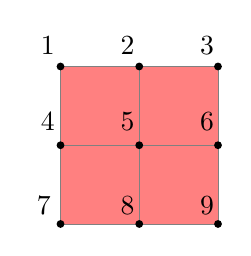
\begin{tikzpicture}
    \fill[red!50] (0,1) rectangle (1,2);
        \fill[red!50] (1,1) rectangle (2,2);
        \fill[red!50] (0,0) rectangle (1,1);
        \fill[red!50] (1,0) rectangle (2,1);
    % Draw the grid
    \draw[step=1cm, gray, very thin] (0,0) grid (2,2);
    
    % Draw the vertices
    \foreach \x in {0,1,2} {
        \foreach \y in {0,1,2} {
            \node[fill=black, circle, inner sep=1pt] at (\x,\y) {};
        }
    }
    % Label the vertices
    \node[anchor=south east] at (0,0) {7};
    \node[anchor=south west] at (1.65,0) {9};
    \node[anchor=north east] at (0.05,2.5) {1};
    \node[anchor=north west] at (1.65,2.5) {3};
    \node[anchor=north] at (0.85,2.5) {2};
    \node[anchor=south] at (0.85,0) {8};
    \node[anchor=west] at (1.65,1.3) {6};
    \node[anchor=east] at (0.05,1.3) {4};
    \node[anchor=center] at (0.85,1.3) {5};
\end{tikzpicture}
%%%  \end{adjustbox}    
\caption{$\LL$.}%
\end{subfigure}%
   \quad
   \begin{subfigure}[b]{0.3\textwidth}
   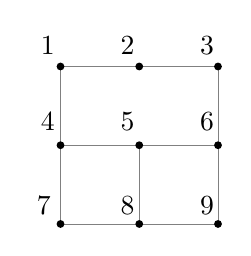
\begin{tikzpicture}
        % Draw and fill the grid squares, except the bottom right one
        % \fill[red!50] (0,1) rectangle (1,2);
        % \fill[red!50] (1,1) rectangle (2,2);
        % \fill[yellow!50] (0,0) rectangle (1,1);
        % \fill[blue!50] (1,0) rectangle(2,1);
        % Bottom right square (1,0) to (2,1) is left empty

        % Draw the grid lines, excluding the edges HI and EI
        % Left vertical grid lines
        \draw[gray, very thin] (0,0) -- (0,2);
        \draw[gray, very thin] (1,0) -- (1,1);
        
        % Right vertical grid line, excluding edge EI
        \draw[gray, very thin] (2,1) -- (2,2);
        
        % Bottom horizontal grid lines
        \draw[gray, very thin] (0,0) -- (1,0);
        \draw[gray, very thin] (1,1) -- (2,1);
        \draw[gray, very thin] (0,1) -- (1,1);
        % \draw[gray, very thin] (1,1) -- (1,2);
        \draw[gray, very thin] (1,2) -- (2,2);

        \draw[gray, very thin] (1,0) -- (2,0);
        \draw[gray, very thin] (2,0) -- (2,1);
        
        % Top horizontal grid lines, excluding edge HI
        \draw[gray, very thin] (0,2) -- (1,2);
        
        % Draw the vertices, excluding the bottom right vertex (2,0)
        \foreach \x in {0,1,2} {
            \foreach \y in {0,1,2} {
                \ifnum\x=2\relax
                    \ifnum\y=0\relax
                        % Skip the vertex (2,0)
                    \else
                        \node[fill=black, circle, inner sep=1pt] at (\x,\y) {};
                    \fi
                \else
                    \node[fill=black, circle, inner sep=1pt] at (\x,\y) {};
                \fi
            }
        }
        
       % Label the vertices
        \node[anchor=south east] at (0,0) {7};
    % \node[anchor=south west] at (1.65,0) {9};
    \node[anchor=north east] at (0.05,2.5) {1};
    \node[anchor=north west] at (1.65,2.5) {3};
    \node[anchor=north] at (0.85,2.5) {2};
    \node[anchor=south] at (0.85,0) {8};
    \node[anchor=west] at (1.65,1.3) {6};
    \node[anchor=east] at (0.05,1.3) {4};
    \node[anchor=center] at (0.85,1.3) {5};
    \node[anchor=south west] at (1.65,0) {9};
    \node[fill=black, circle, inner sep=1pt] at (2,0) {};
    \end{tikzpicture}
    \caption{$\KK$.}
\end{subfigure}%

\caption{The cubical complexes $\KK \hookrightarrow \LL$ associated with Example \ref{ex_cub_1}.}
\label{fig_cubical_cmplexes}
\end{figure}